\section{Experiment Evaluation}

In order to validate the effectiveness of our approach, we simulated 4 stealthy techniques, 23 malicious functions attacks on 100 critical system processes and ten APT attack scenarios:

\begin{itemize}
    \item \textbf{Q1.} How well does our method work, and does it achieve a low false-positive rate and false-negative rate? ((§~\ref{sec-effective})
    \item \textbf{Q2.} What is the time it takes for our method to construct a profile for each process? What is the most time-consuming step in the three-step process profile creation? (§~\ref{sec-eff})
    \item \textbf{Q3.} How does the behavior diverge based on LLM, and how does the validation step optimize the outcome? (§~\ref{sec-ab-study})
    \item \textbf{Q4.} How can we validate the accuracy of these explanations using our method? (§~\ref{sec-explanation-val})
    \item \textbf{Q5.} Is it common for real-world APT attacks to disguise their processes in various ways? (§~\ref{sec-real-world})
\end{itemize}
All experiments are performed on a server with Intel Xeon E5-2620 v4 CPUs @ 2.10GHz, 64 GB physical memory, and an NVIDIA Tesla V100 GPU. The OS is Ubuntu 16.04.3 LTS.
We implemented our system by calling OpenAI's GPT-4 API with a temperature setting of 0.5.
We develop \tool in 3.53K lines of C++ code and 10K lines of Python code.
The C++ code in the project is utilized for the generation of malicious attacks, while the Python code is employed for data preprocessing, building process profiles, and threat detection.


\subsection{Implementation}
We present important technical details in the implementation.

\subsubsection{System Auditing Collection}
Although \tool can handle input from Linux and Windows systems, our evaluation focuses primarily on Windows events. Because most of our benign deployment environment consists of Windows-based hosts, and sophisticated malware is mostly designed for Windows platforms, this is largely due to the fact that we have a benign deployment environment. We use Sysmon, Windows' sophisticated log collection tool, to collect provenance data from these systems. System logs are captured thoroughly and exhaustively by leveraging Sysmon's default settings.

\subsubsection{Attack Datasets}

To address the challenges, we approached the problem from three distinct angles: expanding coverage of malicious functionalities and the ATT\&CK framework, employing advanced stealthy techniques, and simulating genuine APT attacks.

We executed our APT attack simulations in three steps:
\begin{itemize}
    \item  \textbf{Enhancing Malicious Functionalities:} In order to simulate a wider range of malicious activities, we handcrafted 14 malicious functions in C++, including BypassUAC, Encryption, File Monitor, Keyboard Monitor, and Privilege Escalation. In addition, we implemented nine different TTP attacks using well-known hacker utilities like Caldera. Using C++ and Caldera methodologies, we achieved 23 distinct malicious functions. APT attacks take place at various stages, including Initial Access, Privilege Escalation, Information Gathering, Defense Evasion, and ensuring Persistence.
    \item \textbf{Employing Stealth Techniques:} We incorporated four stealth methods: Process Masquerade, Process Hollow, Process Injection, and DLL Side-Loading. By combining these stealth techniques with the 23 malicious functionalities, a variety of attack variants can be created. Process Masquerade and Process Hollow hide malicious process names, while Process Injection and DLL Side-Loading hide malicious DLLs.
    \item \textbf{Simulating Real-world APTs:} In order to enhance the authenticity of our simulations, we developed ten APT attack scenarios based on an analysis of real-world Advanced Persistent Threat activities. During a controlled testbed environment, audit logs were produced. We crafted ten simulated APT attack narratives using the four stealth techniques from the second step and the 23 malicious functionalities from the first step.
\end{itemize}

\noindent
{\bf Real-world datasets.} Using real-world datasets, we aimed to validate the frequency of obfuscation techniques such as name masquerading in authentic APT attacks and associated malicious software; to this end, we collected publicly available APT attack simulation datasets alongside malware samples like CozyCar,  callium, and Kevin etc. which are known to employ techniques like name masquerading and process injection;  APT29 poses as \textit{python.exe}, \textit{rar.exe}, and \textit{accesschk.exe}; furthermore, they utilize DLL Side-Loading, specifically by loading a malicious \textit{mso.dll} file, with comprehensive details showcased in the subsequent Table~\ref{tab:real_world}. We will delve into the specifics of how we utilized real-world datasets to validate the efficacy of our approach in Section~\ref{sec-real-world}.

\noindent
{\bf Label.}
By using our knowledge of attack workflow, we manually label the ground truth of interactions through their relation to attacks, as we are aware of how attacks are executed.


\subsubsection{Normal Datasets}
To validate the false positive rate of our methodology, we sourced a publicly available benign dataset from GitHub\cite{evtx-baseline2022}. This dataset encompasses logs generated from routine user activities across various Windows operating systems, including Windows 7, Windows 10 and Windows 11. The logs from this dataset cover the 13/47/52 processes we use to construct process profiles.

\begin{figure}[h]
    \centering
      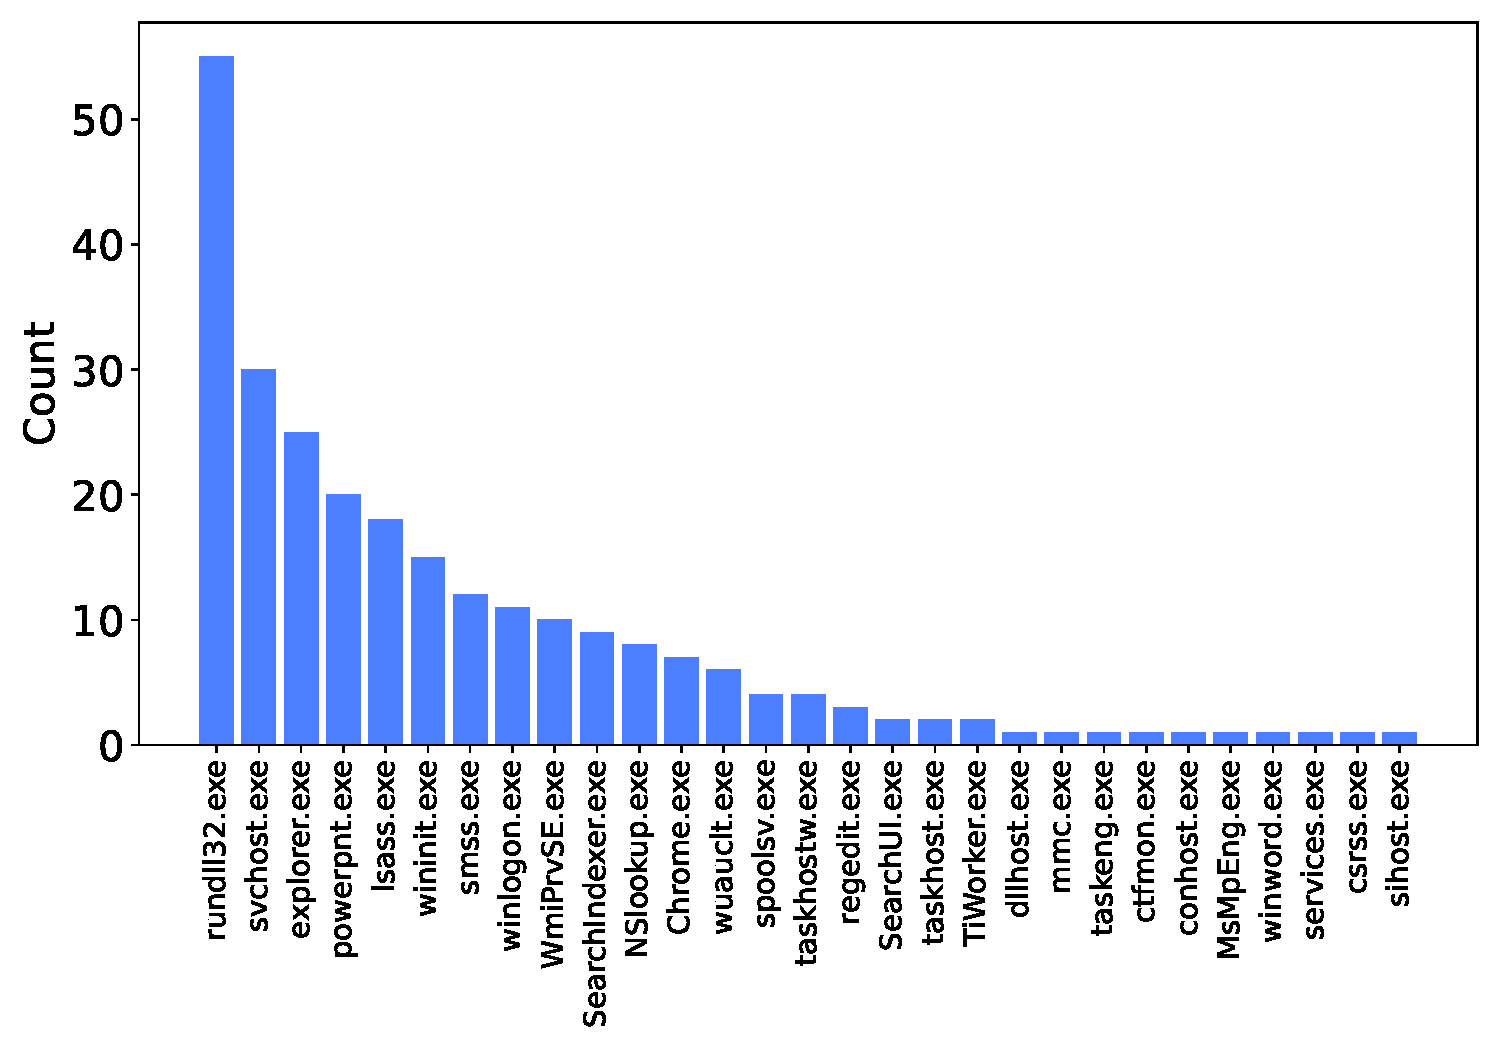
\includegraphics[width=0.45\textwidth]{figs/process.pdf}
    \caption{Comparison of attack frequencies for different processes based on the official MITRE website.}
    \label{fig-process}
\end{figure}

\subsubsection{Process Classification}

In order to construct a comprehensive analysis framework, we strategically selected 100 pivotal processes for examination. The selection criteria encompassed multiple dimensions, including: 1) Core system processes that are integral to system functionality; 2) Processes highly associated with security mechanisms; and 3) Processes commonly utilized by system administrators. Additionally, we integrated an assessment of processes that are frequently targeted in cyber-attacks, based on statistical analysis derived from MITRE's official website as shown in Figure~\ref{fig-process}


\newcommand{\colorbar}[1]{%
    \begin{tikzpicture}
        \definecolor{mycolor}{RGB}{255,204,204}
        \fill[mycolor] (0,0) rectangle (#1/100*0.7, 0.5); %0.7 is the width, adjust as needed
        \draw[black] (0,0) rectangle (0.7,0.5);
    \end{tikzpicture}
}


We highlight the two most common processes: svchost.exe and rundll32.exe:
\begin{itemize}
    \item \textbf{\textit{Svchost.exe} processes}. svchost.exe is a Windows system utility that runs multiple services from dynamic link libraries (.dll files). Given its trusted status and constant presence, adversaries often mimic svchost.exe for attacks. The behavior tree for svchost.exe, constructed based on our approach, is shown in the Figure~\ref{fig:behavior-tree}.
    \item \textbf{\textit{Rundll32.exe} processes}. \textit{rundll32.exe} loads specific functions from .dll files. Unlike \textit{svchost.exe}, it's more vulnerable, as attackers can create their own .dll for it. Due to its exploitability, \textit{rundll32.exe} is a prime target for malware impersonation. 
\end{itemize}



\subsection{Effectiveness}
\label{sec-effective}

\begin{figure*}
  \centering
  \begin{minipage}[b]{0.65\textwidth} 
  \begin{subfigure}{.5\textwidth}
      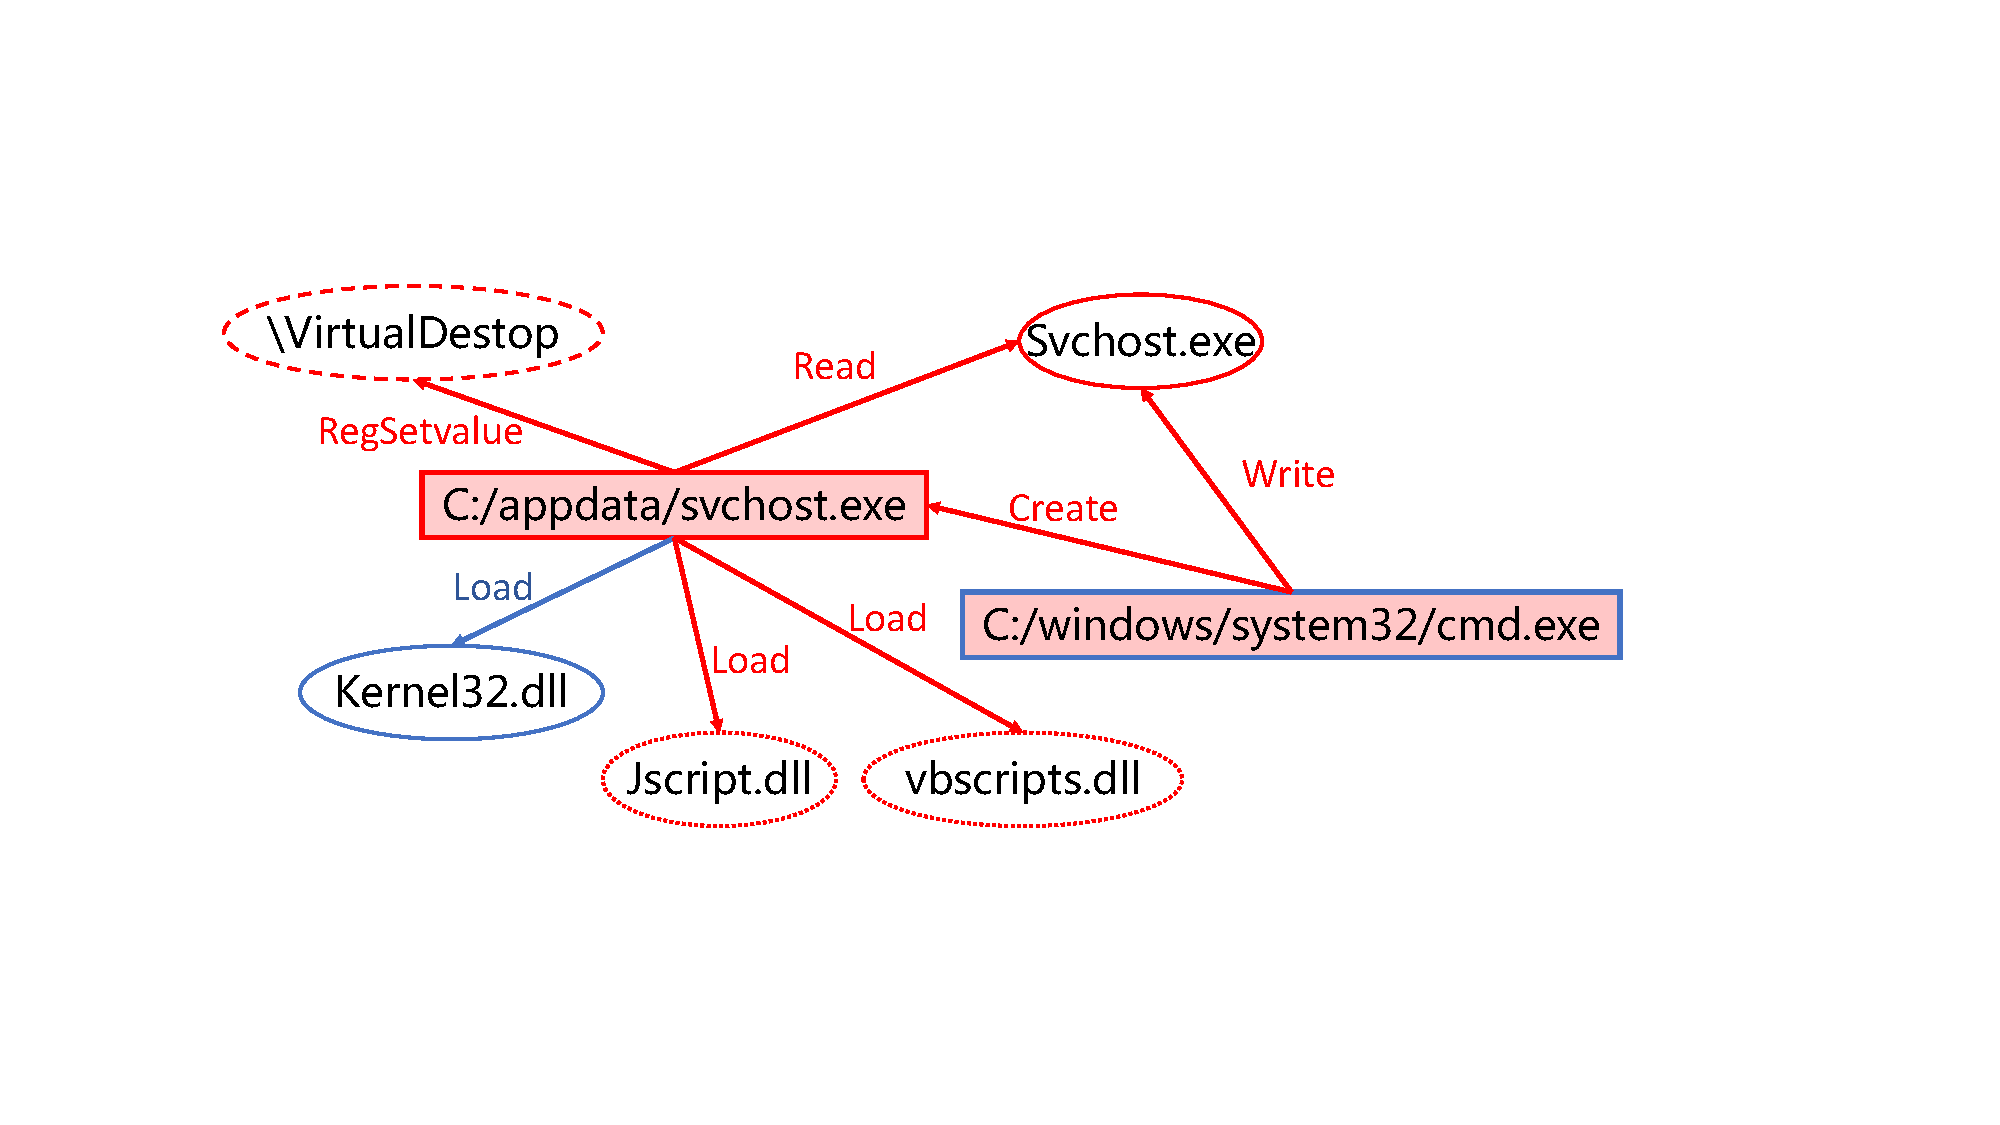
\includegraphics[width=\textwidth]{figs/Process Masquerade.pdf}
      \caption{Process Masquerade}
      \label{fig:process_mas}

  \end{subfigure}
  \hfill
  \begin{subfigure}{.5\textwidth}
      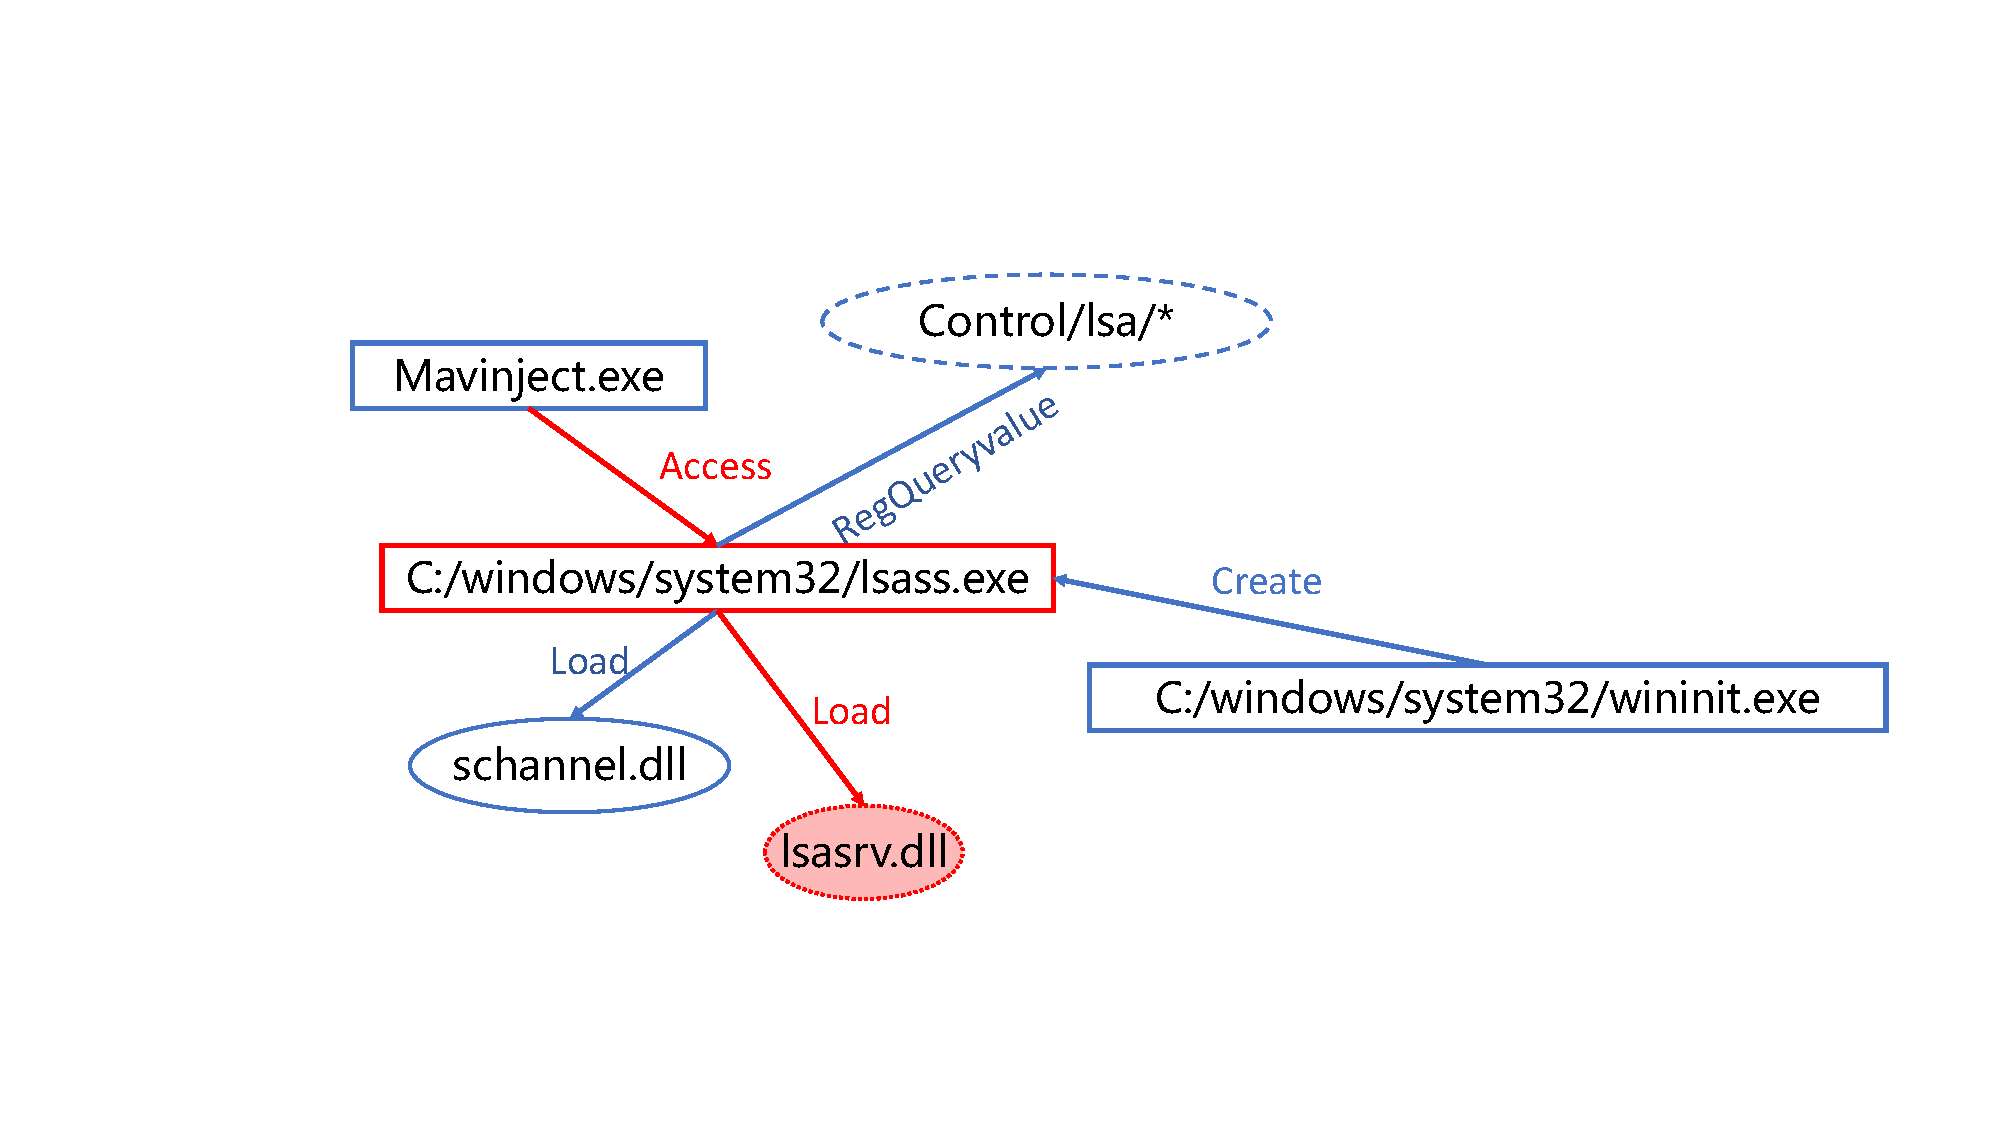
\includegraphics[width=\textwidth]{figs/process_injection.pdf}
      \caption{Process Injection}
      \label{fig:process_inj}

  \end{subfigure}

  \begin{subfigure}{.5\textwidth}
      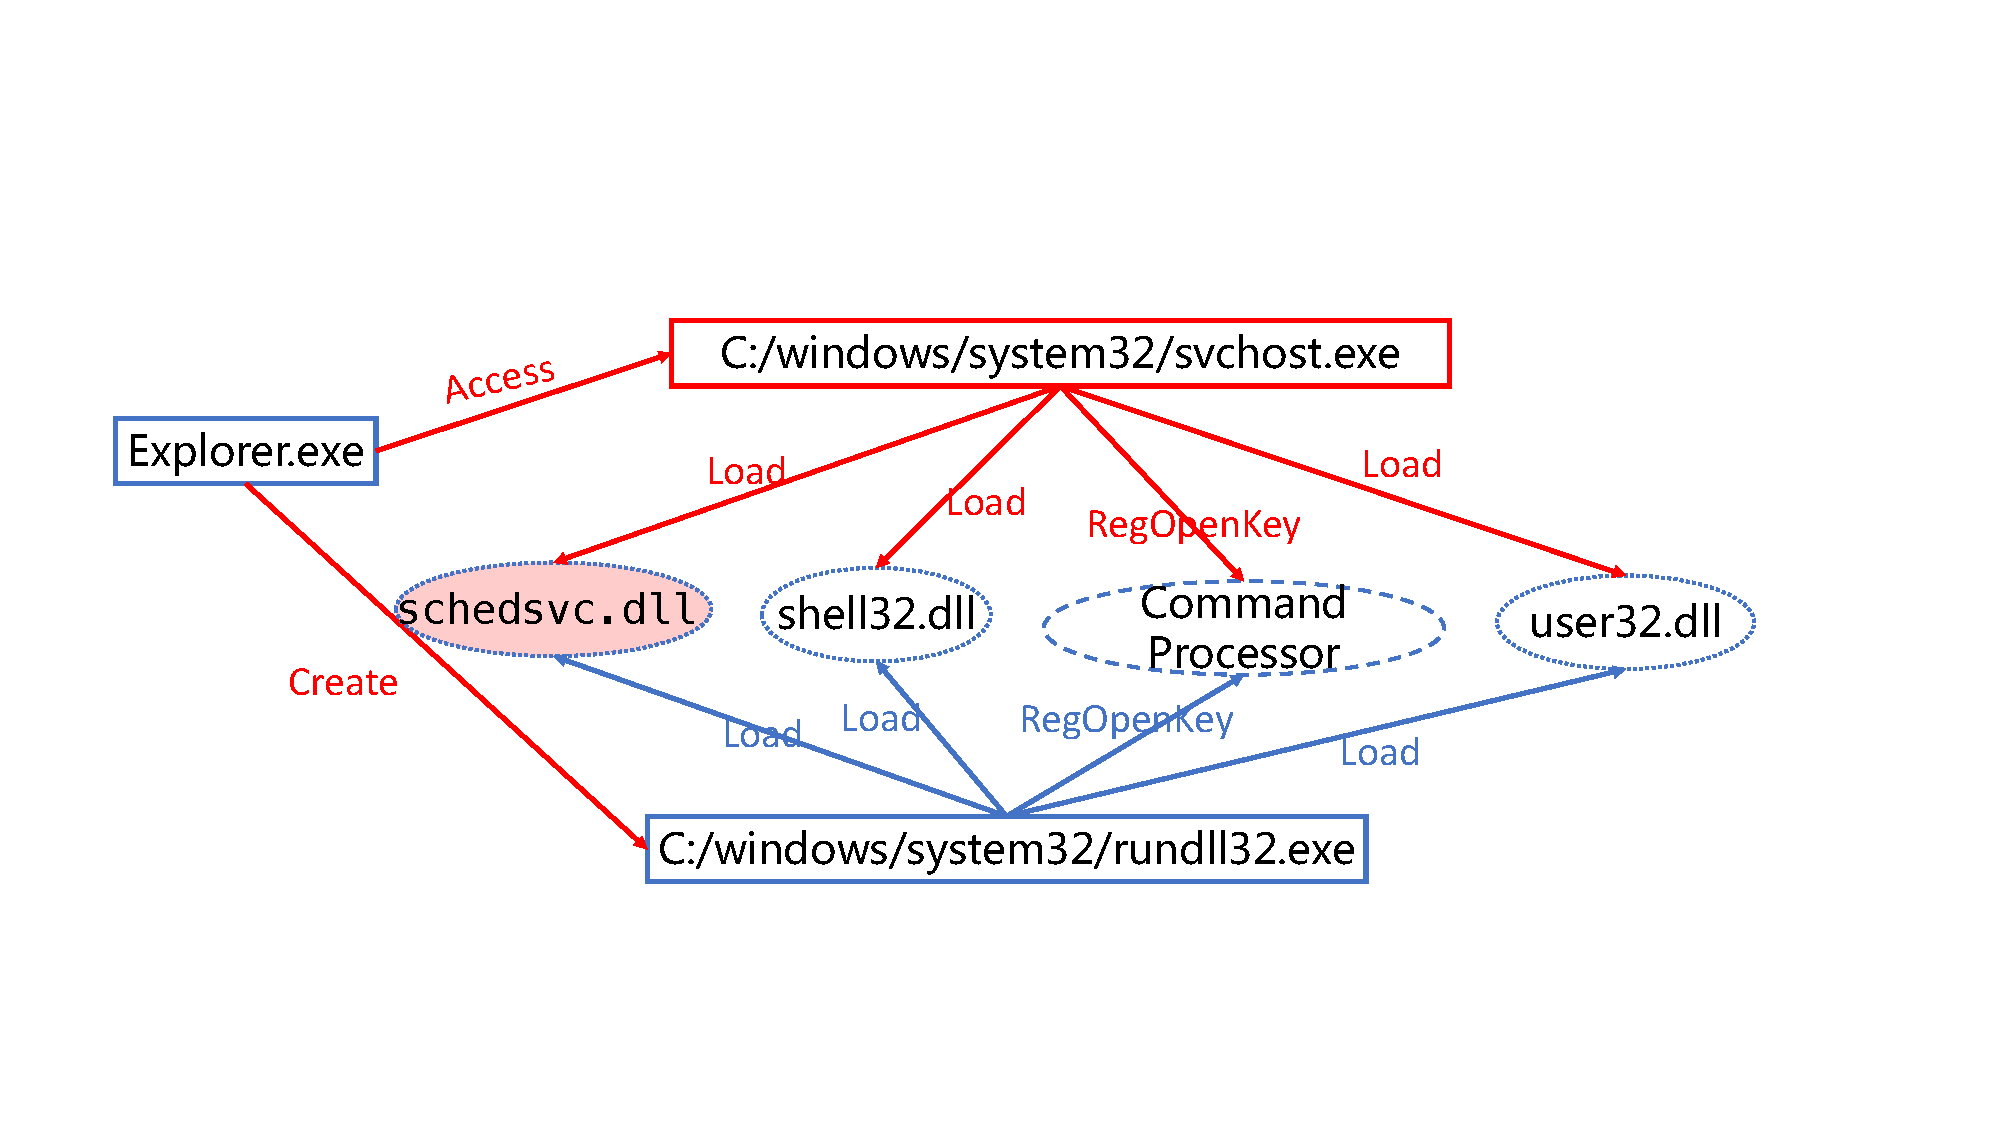
\includegraphics[width=\textwidth]{figs/Process Hollow.pdf}
      \caption{Process Hollow}
      \label{fig:hollow}

  \end{subfigure}
  \hfill
  \begin{subfigure}{.5\textwidth}
      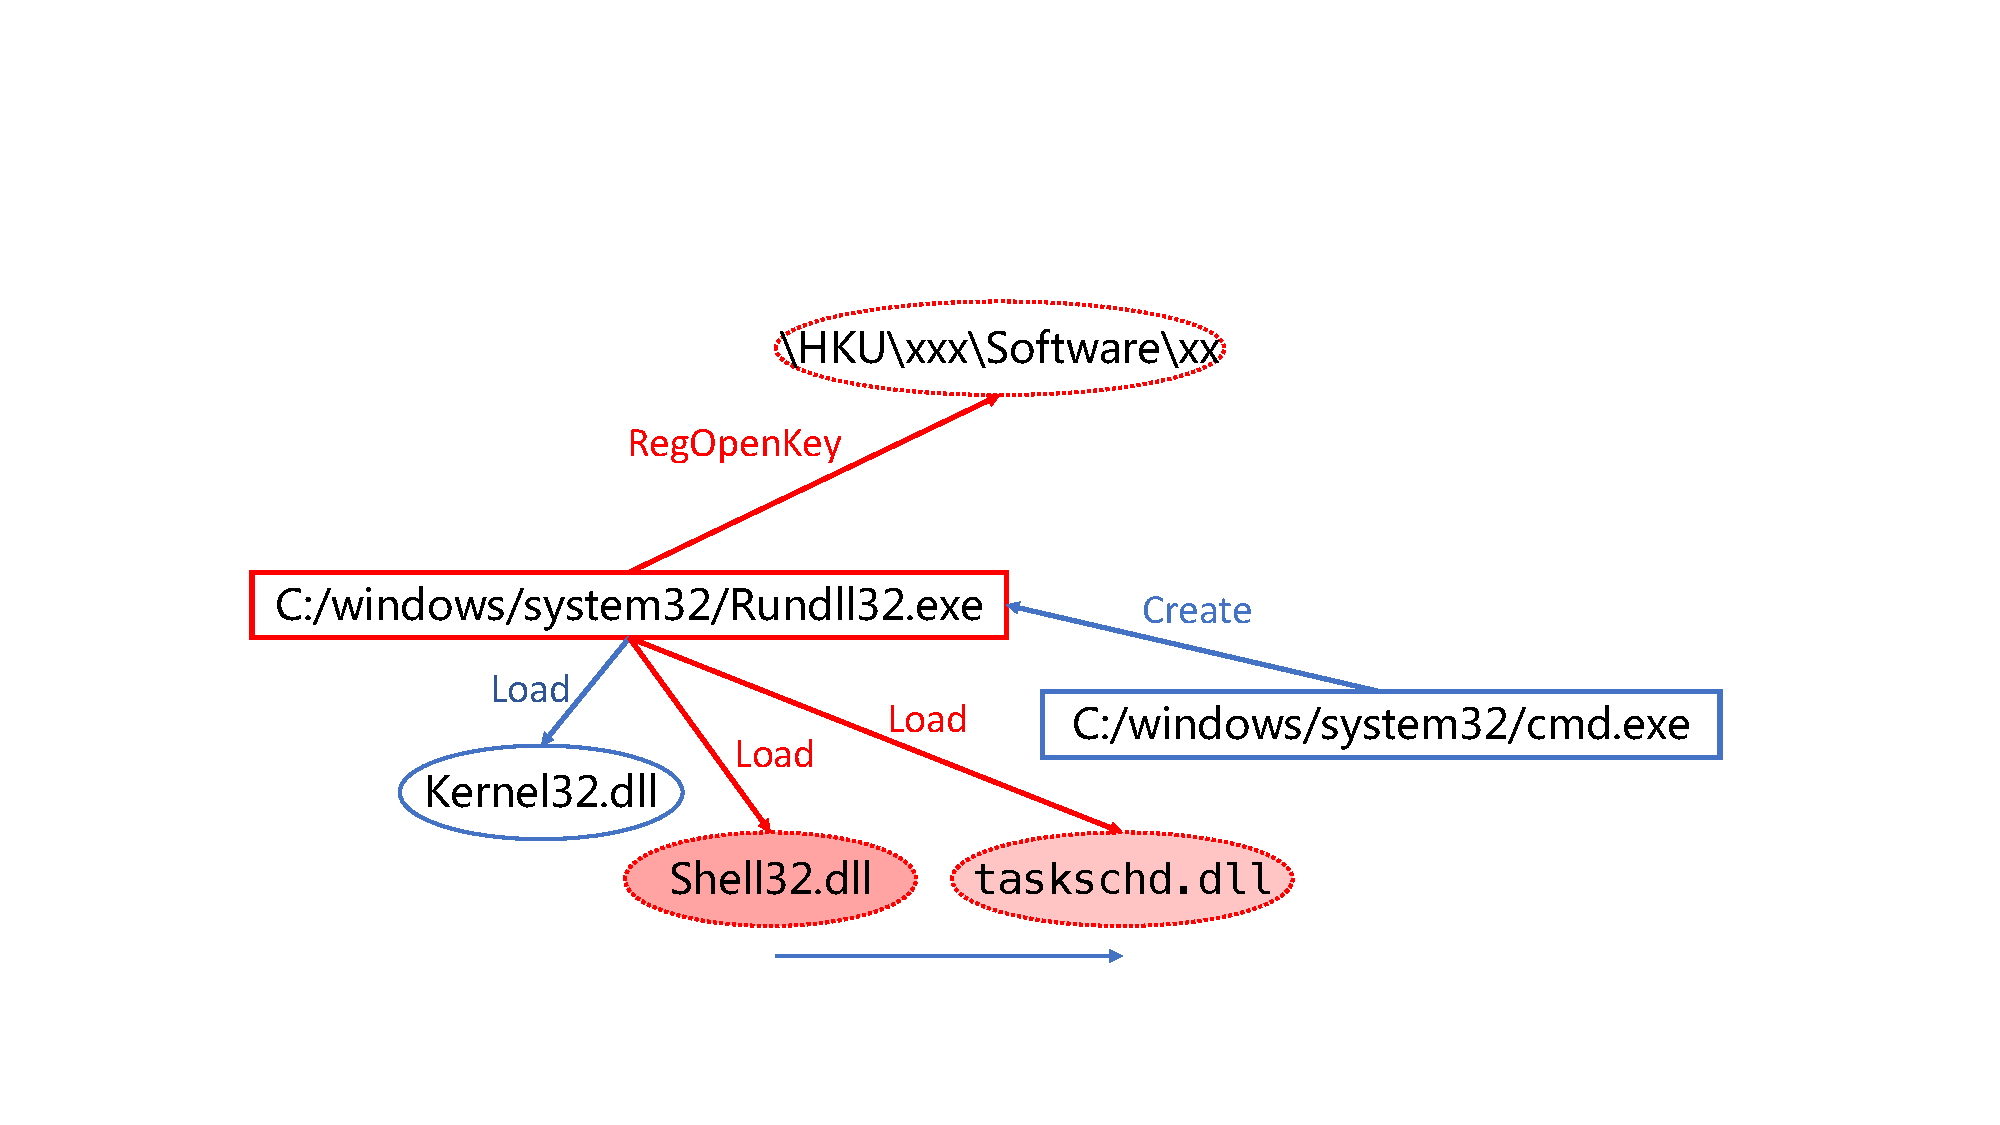
\includegraphics[width=\textwidth]{figs/Dll Side-Loading.pdf}
      \caption{Dll Side-Loading}
      \label{fig:side-load}
  \end{subfigure}

  \centering
 \caption{Each solid node in the graph represents detected signal, which has violated various constraints.}
\end{minipage}
\hfill
\begin{minipage}[b]{0.34\textwidth} 

  \begin{subfigure}{.99\textwidth}
      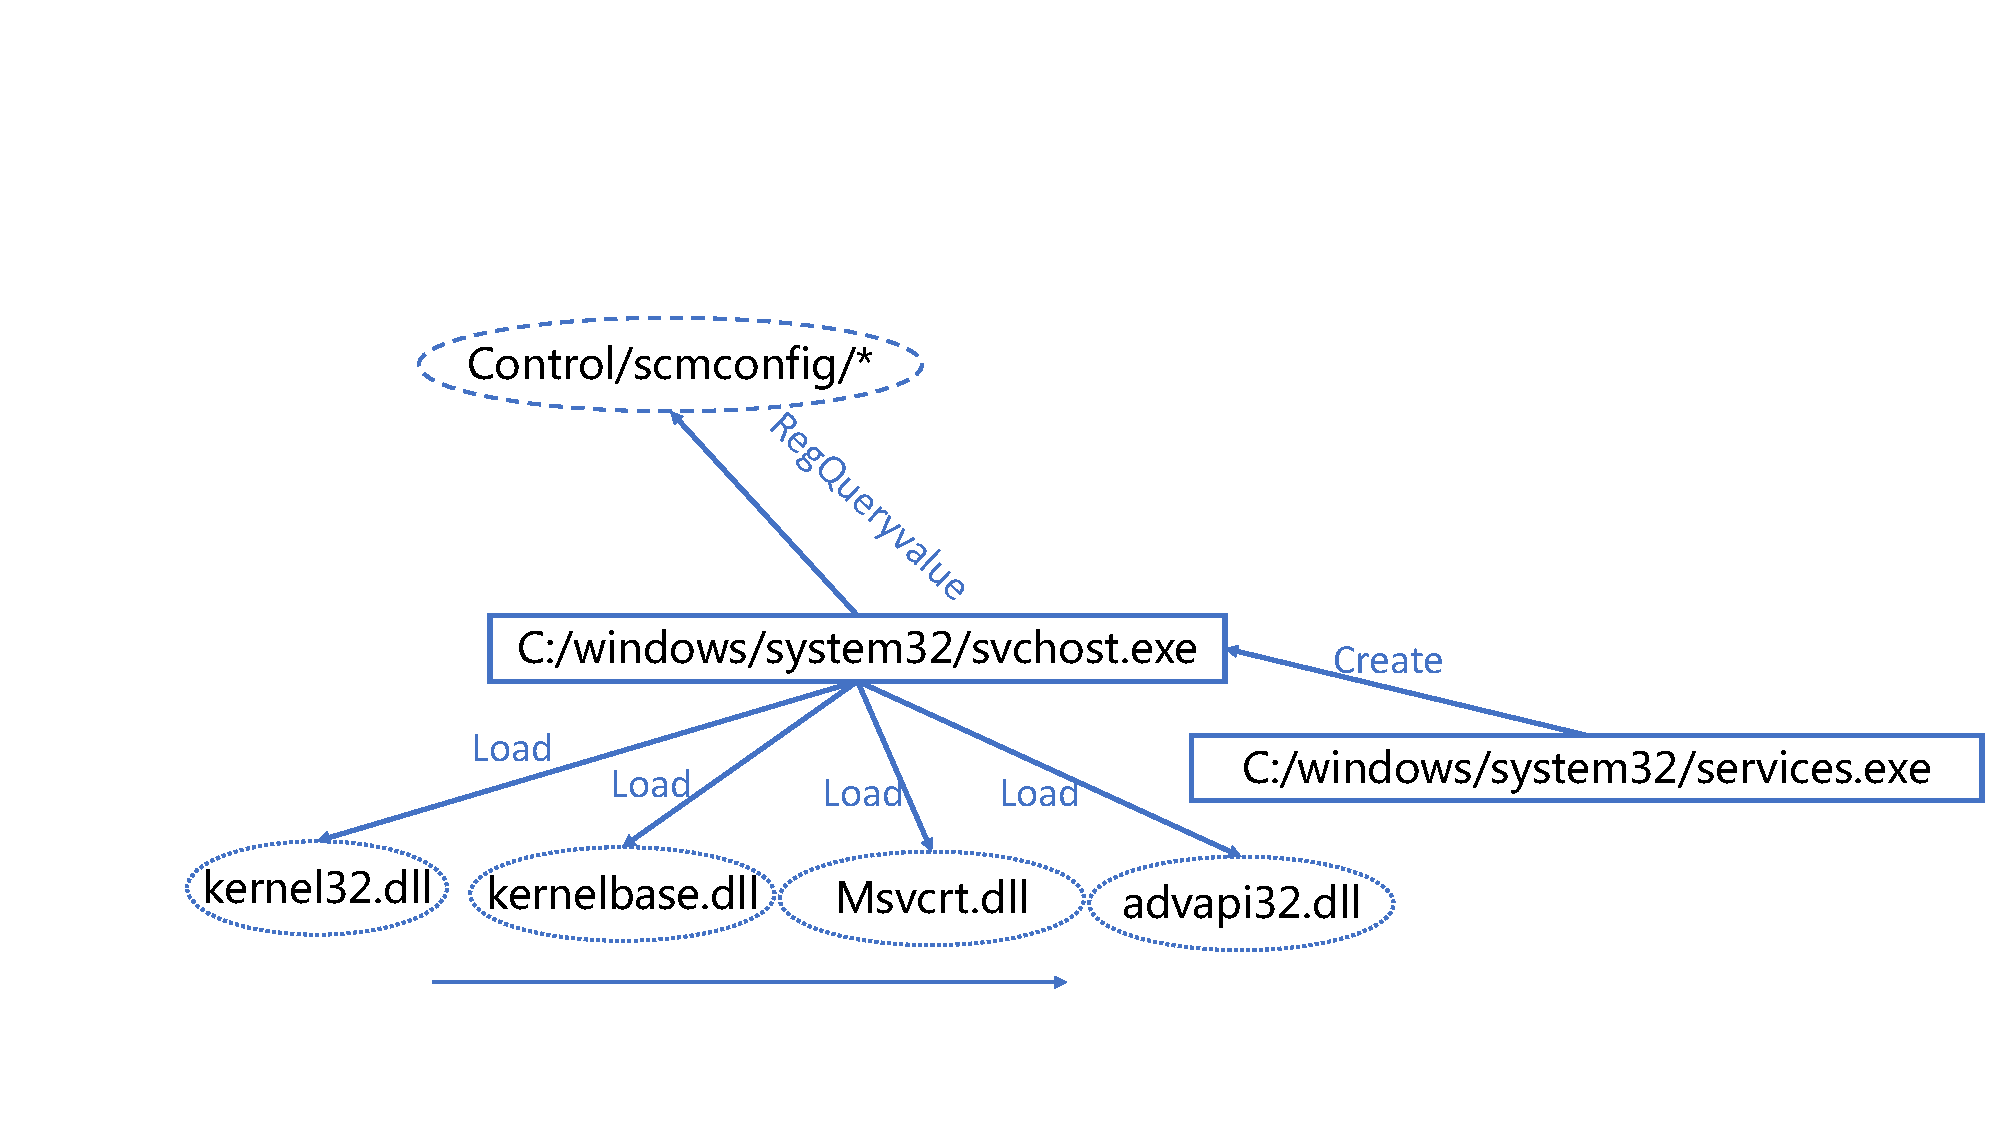
\includegraphics[width=\textwidth]{figs/svchost.pdf}
      \caption{Svchost Constraints}
      \label{fig:svc-cons}
  \end{subfigure}
  \hfill
  -\vspace{0.9cm}
  \begin{subfigure}{.99\textwidth}
      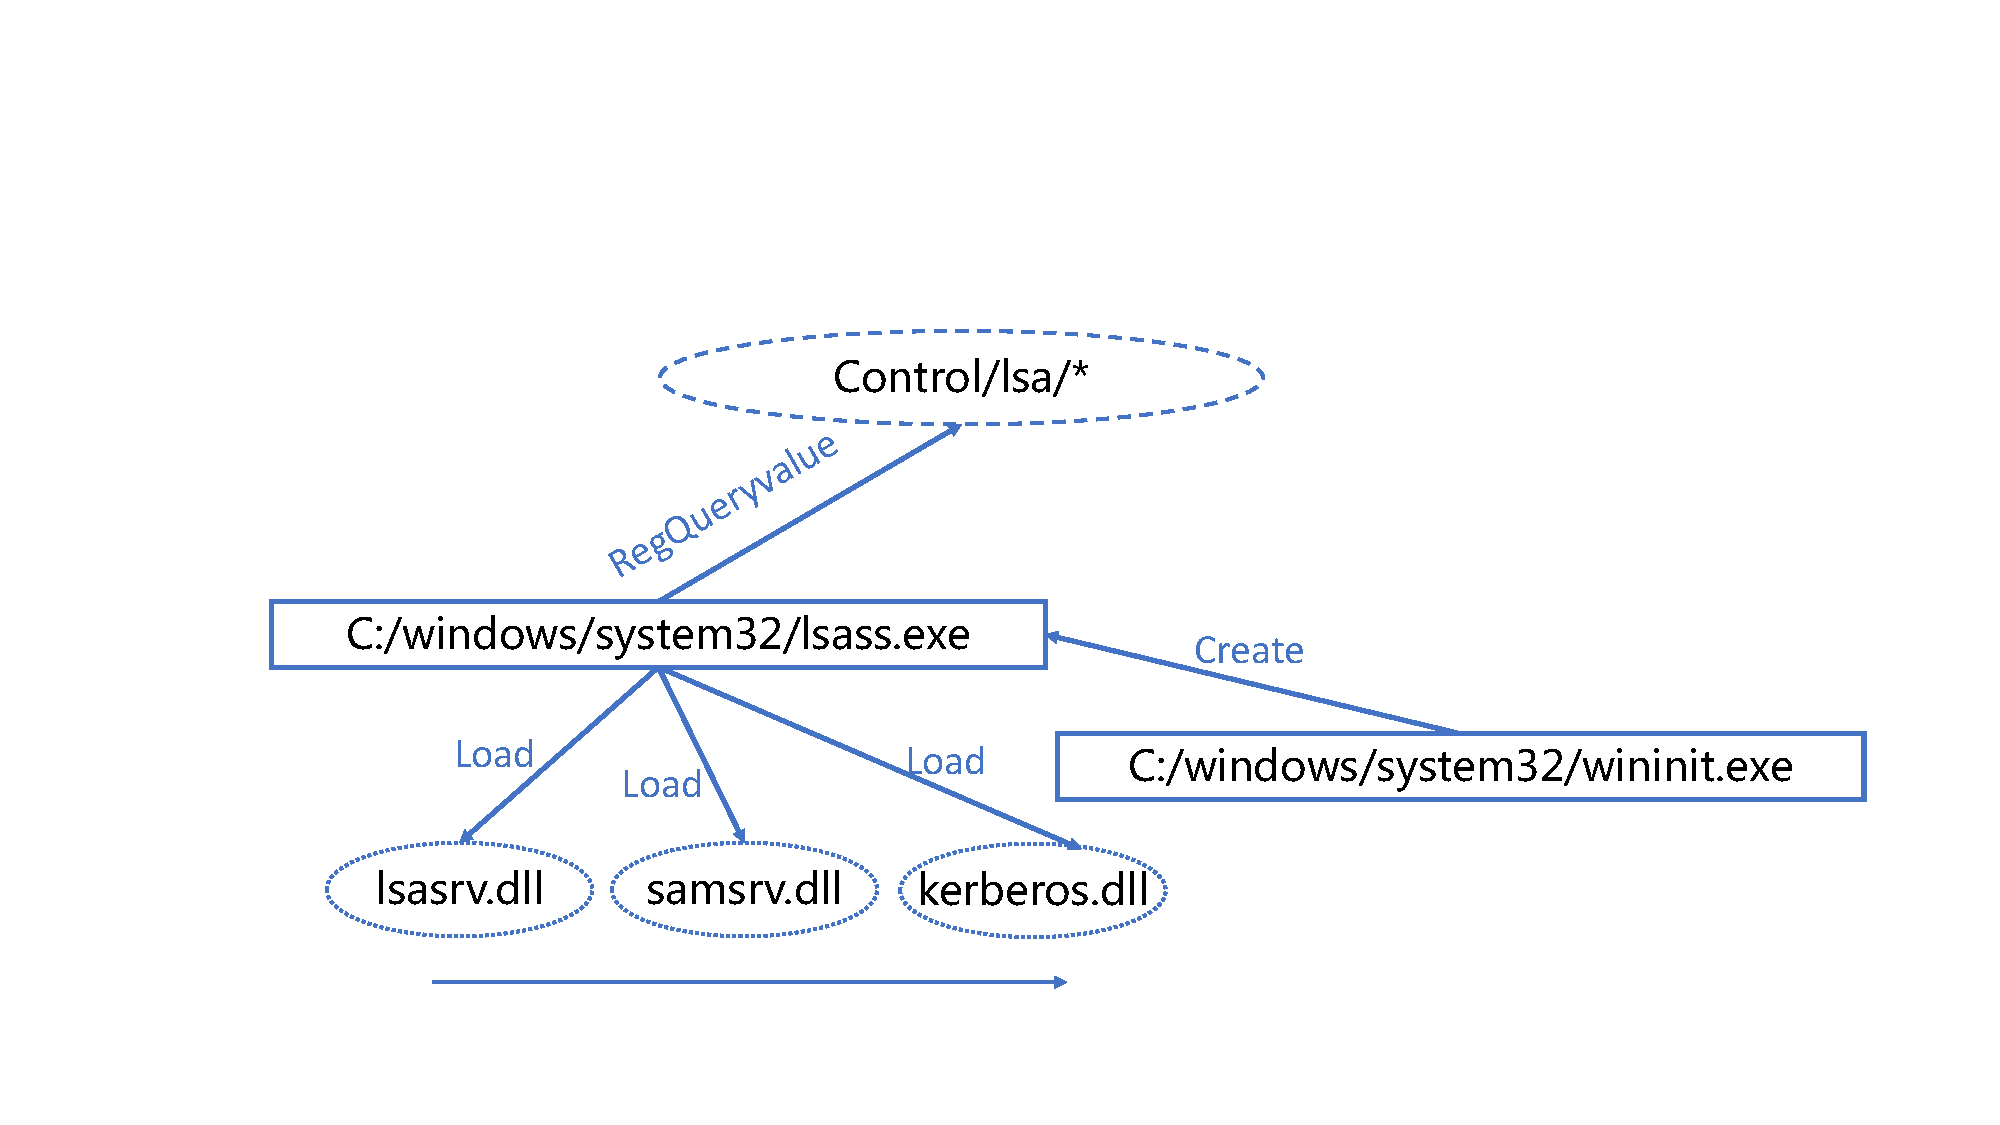
\includegraphics[width=\textwidth]{figs/lsass.pdf}
      \caption{Lsass Constraints}
      \label{fig:lsass-cons}
  \end{subfigure}
\caption{Constraints}
\label{fig-fdh}
\end{minipage}
\end{figure*}

\subsubsection{Evaluation on Attack for Various Processes}
We launched attacks on 100 system processes using 4 stealthy techniques, targeting 10 malicious functionalities. As illustrated in the Table~\ref{table:eva-attack}, it's evident that our method achieves a low false negative rate. However, some errors still persist, which we intend to delve into further.

\begin{table*}[h!]
    \centering
    \begin{tabularx}{\textwidth}{|X|X|X|X|X|X|X|X|X|X|X|}
        \hline
        & \textbf{BU} & \textbf{C} & \textbf{FM} & \textbf{FS} & \textbf{ST} & \textbf{PE} & \textbf{KM} & \textbf{FA} & \textbf{SE} & \textbf{E} \\
        \hline
\multicolumn{1}{|l|}{\textbf{PM}} & \multicolumn{1}{l|}{59/60}   & \multicolumn{1}{l|}{59/60}  & \multicolumn{1}{l|}{59/60}   & \multicolumn{1}{l|}{59/60}   & \multicolumn{1}{l|}{59/60}   & \multicolumn{1}{l|}{59/60}   & \multicolumn{1}{l|}{59/60}   & \multicolumn{1}{l|}{59/60}   & \multicolumn{1}{l|}{59/60}   & \multicolumn{1}{l|}{59/60}  \\ \hline
\multicolumn{1}{|l|}{\textbf{PH}} & \multicolumn{1}{l|}{59/60}   & \multicolumn{1}{l|}{57/60}  & \multicolumn{1}{l|}{57/60}   & \multicolumn{1}{l|}{58/60}   & \multicolumn{1}{l|}{58/60}   & \multicolumn{1}{l|}{59/60}   & \multicolumn{1}{l|}{57/60}   & \multicolumn{1}{l|}{57/60}   & \multicolumn{1}{l|}{59/60}   & \multicolumn{1}{l|}{60/60}  \\ \hline
\multicolumn{1}{|l|}{\textbf{PI}} & \multicolumn{1}{l|}{56/60}   & \multicolumn{1}{l|}{55/60}  & \multicolumn{1}{l|}{57/60}   & \multicolumn{1}{l|}{59/60}   & \multicolumn{1}{l|}{57/60}   & \multicolumn{1}{l|}{58/60}   & \multicolumn{1}{l|}{59/60}   & \multicolumn{1}{l|}{57/60}   & \multicolumn{1}{l|}{57/60}   & \multicolumn{1}{l|}{58/60}  \\ \hline
\textbf{DLL}                      & 59/60                        & 58/60                       & 57/60                        & 57/60                        & 59/60                        & 56/60                        & 57/60                        & 57/60                        & 58/60                        & 56/60                       \\ 
        \hline
    \end{tabularx}
    \caption{Detection of Process Count for Various Techniques and Malicious Activities.}
    \smallskip
    \small \textit{Abbreviations: BU - BypassUAC, C - Compress, FM - File Monitor, FS - File Scan, ST - Scheduled Task, PE - Privilege Escalation, KM - Keyboard Monitor, FA - Forced Authentication, SE - Service Execution, E - Exfiltration, PM - Process Masquerade, PH - Process Hollow, PI - Process Injection, DLL - DLL Side-Loading}
    \label{table:eva-attack}
\end{table*}
\smallskip
\noindent
{\bf Analysis of False Negatives.}
We discovered two primary reasons for these errors after thoroughly examining the incorrect cases:
\begin{itemize}
    \item \textbf{Some stealthy attack does not violate a constraint}: There are some stealthy attacks that do not violate any established constraints. For example, some rundll32.exe attack operates within its legitimate bounds. Live-off-ground attacks leverage the normal functionality of legitimate programs for malicious purposes.

    \item \textbf{Insufficient Knowledge for Certain Processes}:  The internal knowledge of the large language model is limited for some processes. Consider the process \textit{amdfendrsr.exe}(AMD Crash Defender Service), which is a core system process associated with the executable file \textit{amdfendrsr.exe}. The existing knowledge base lacks comprehensive details on this process. Consequently, the constructed profile results in weak constraints, which render the model incapable of detecting attacks that violate the \textit{amdfendrsr.exe} process constraints.
\end{itemize}
Given these findings, it's imperative to address these gaps to enhance the efficacy of our attack detection approach.


\subsubsection{Evaluation on Normal Workloads}
As previously mentioned, we sourced logs from different Windows versions from GitHub\cite{evtx-baseline2022}, specifically Windows 7, Windows 10, and Windows 11. These logs were collected from various users performing an array of routine operations. We utilized these logs to assess the false positive rate (i.e., false alarms) of our method in these scenarios.

In the Windows 7 scenario, our investigation encompassed 13 processes from our list, which manifested in 159 distinct entities due to multiple entities associated with a single process name. For Windows 10, we analyzed 47 processes (564 entities), and for Windows 11, we focused on 52 processes (1137 entities).

\begin{figure}[h]
    \centering
      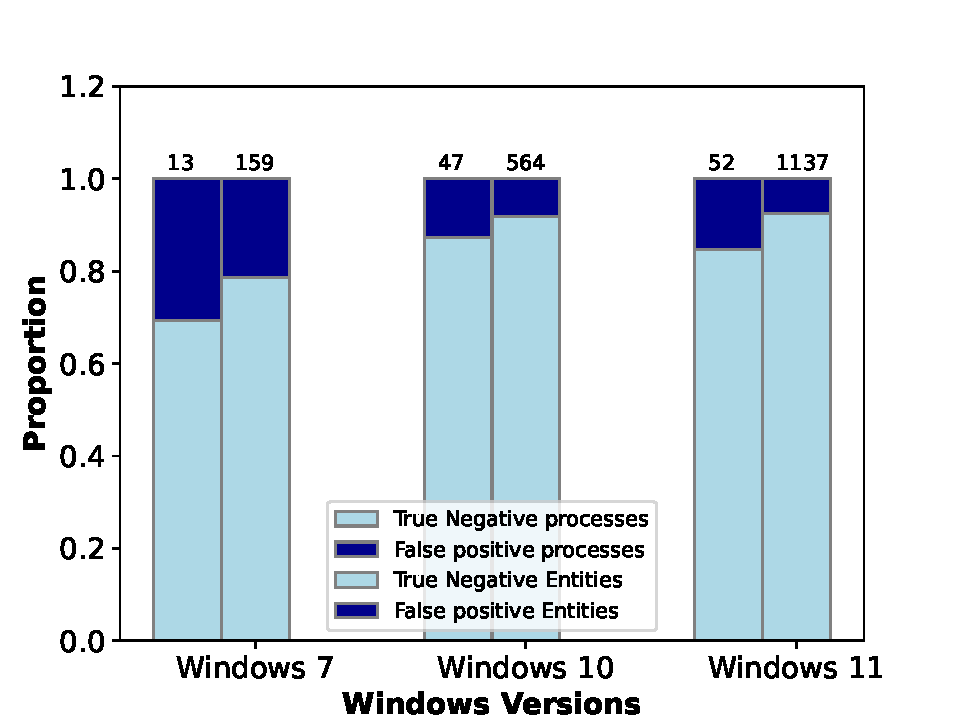
\includegraphics[width=0.49\textwidth]{figs/normal_chart.pdf}
    \caption{Evaluation on Normal Workloads.}
    \label{fig-eva-normal}
\end{figure}

\smallskip
\noindent {\bf Analysis of False Positives.}
After a detailed analysis of the various causes of false positives, we identified the following key issues:

\begin{itemize}
    \item \textbf{Uniformity in LLM's Results:} The LLM system tends to offer overly single results. For instance, the parent processes of \textit{C:/Windows/explorer.exe} can vary widely, including options like \textit{C:/Windows/explorer.exe} itself and \textit{C:/Windows/System32/svchost.exe}. However, LLM only provides feedback for \textit{userinit.exe}. This means that any normal process not having \textit{userinit.exe} as its parent process gets flagged incorrectly. This issue is also evident in processes like \textit{dllhost.exe} and \textit{conhost.exe} which can have multiple parent processes.
    \item \textbf{Overconfidence in LLM's Analysis:} For some events that might be absent in a few scenarios, the LLM tends to be overly confident. A case in point is the event \textit{(lsass.exe RegSetValue,hklm/system/currentcontrolset/control/lsa/*)}. While this event is expected to occur in the majority of scenarios, there are specific situations where it might not manifest. As a result, standard events get flagged erroneously. Another example includes a set of three events:\textit{(lsass.exe,Load Image,c:/windows/system32/lsasrv.dll->lsass.exe,Load Image,c:/windows/system32/samsrv.dll->lsass.exe,Load Image,c:/windows/system32/kerberos.dll)}. Typically, these events appear together. However, the event associated with kerberos.dll can sometimes be absent or loaded ahead of time. Consequently, having a stringent expectation for normal programs to execute in a specific order leads to false alarms.
    \item \textbf{Operating System Version Discrepancies:} Our process profile was built based on Windows 10 scenarios. As a result, while false positives are lower in a Windows 10 environment, they're notably higher for Windows 7. This is because Windows 10, being a newer version compared to Windows 7, has undergone changes in process behavior. For instance, in Windows 7, a single \textit{svchost.exe} might host multiple services. In contrast, in Windows 10, it can only host one. Consequently, profiles constructed for Windows 10 tend to have higher false positives when applied to Windows 7.
\end{itemize}


\subsubsection{Evaluation on Simulated APT scenarios}
We construct 10 simulated APT attack scenarios by combining single attack behavior and compare our method against four state-of-the-art techniques. By analyzing cases where current methods exhibit false positives, we aim to explain why these methods might produce false positives.

\begin{figure}[ht]
    \centering
      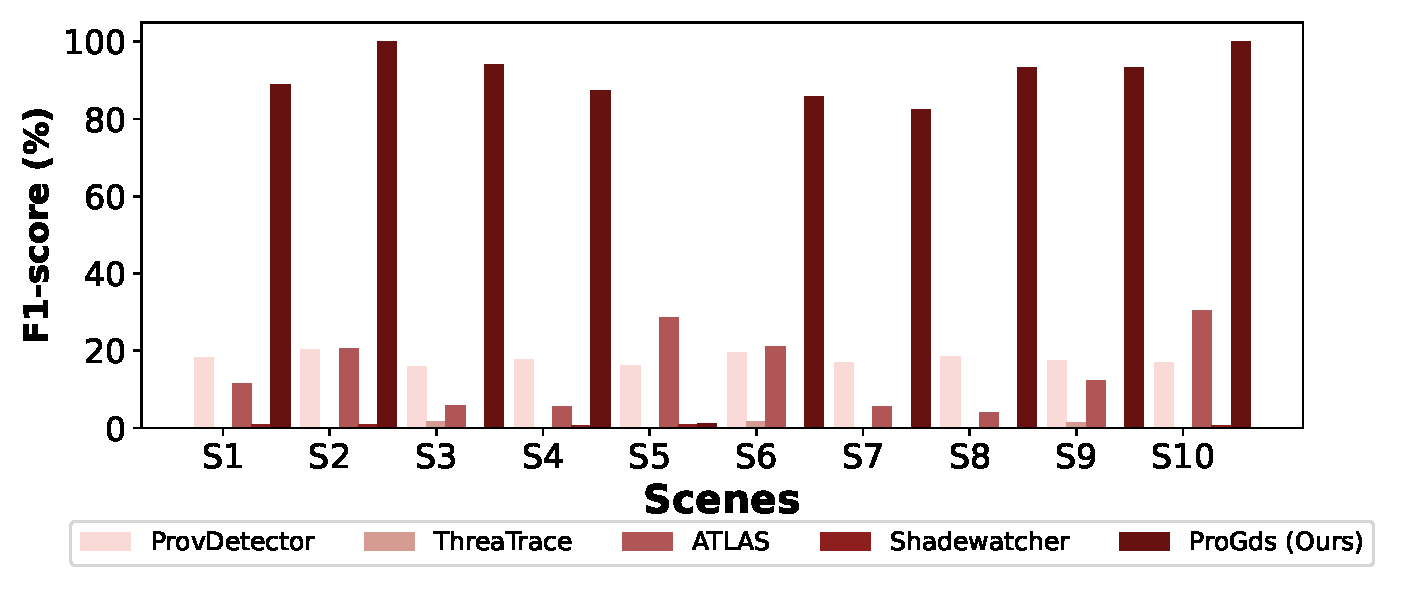
\includegraphics[width=0.49\textwidth]{figs/compare.pdf}
    \caption{Evaluation on Simulated APT scenarios.}
    \label{fig-eva-apt}
\end{figure}

\begin{itemize}
    \item \textbf{ThreaTrace}\cite{wang2022threatrace} An algorithm that constructs unique models for each type of node within a provenance graph aims to identify anomalies at the node level. Since this is a method based on anomalous nodes, we can compare the final false positive and false negative rates fairly.
    \item \textbf{ATLAS}\cite{alsaheel2021atlas} Uses graphs to derive attack and non-attack sequences, as well as sequence models to discern attack patterns. we compared the detection effect at the node level because our method is process-centered.
    \item \textbf{Shadewatcher} \cite{zengy2022shadewatcher} We have adapted the method originally designed for information flow for our comparative analysis. First, we use Shadewatcher's embedding method to get the node's vector, as soon as the embedding of the node is obtained, we use LOF anomaly detection to determine the detection rate of abnormal nodes.
    \item \textbf{ProvDetector.} A method analogous to ours is ProvDetector\cite{wang2020you}. It identifies malware by analyzing the provenance graph. In order to detect malware, it transforms paths within the graph into embedded representations and then uses the Local Outlier Factor technique. To evaluate the effectiveness of our method against ProvDetector, we analyzed results based on event investigation.
\end{itemize}


\begin{table}
    \centering
    \small 
    \begin{tabular}{|c|c|c|c|c|}
        \hline
        \multicolumn{1}{|c|}{Attack ID} & \multicolumn{2}{c|}{Process} & \multicolumn{2}{c|}{Entity} \\
        \cline{2-5}
        & \#Attack & \#Non-attack & \#Attack & \#Non-attack \\
        \hline
        S-1 & 8 & 738 & 41 & 2286 \\
        S-2 & 8 & 939 & 41 & 2669 \\
        S-3 & 9 & 1003 & 43 & 2704 \\
        S-4 & 7 & 713 & 18 & 2051 \\
        S-5 & 9 & 1134 & 45 & 3038 \\
        S-6 & 7 & 893 & 38 & 2277 \\
        S-7 & 8 & 718 & 21 & 2101 \\
        S-8 & 8 & 1092 & 42 & 2951 \\
        S-9 & 8 & 1090 & 42 & 2699 \\
        S-10 & 7 & 748 & 21 & 2157 \\
        Avg. & 8 & 907 & 35 & 2493 \\
        \hline
    \end{tabular}
    \caption{Process-based and entity-based investigation results.}
\end{table}

\begin{table}[ht]
\centering
\begin{tabular}{|l|c|c|c|}
\hline
\textbf{Method} & \textbf{P(Avg.)} & \textbf{R(Avg.)} & \textbf{F1(Avg.)} \\
\hline
ProvDetector & 17.82\% & 47.58\% & 47.85\% \\
ThreaTrace & 1.01\% & 35.84\% & 2.00\% \\
ATLAS & 9.63\% & 57.83\% & 14.68\% \\
Shadewatcher & 6.52\% & 0.20\% & 0.41\% \\
\tool & 94.44\% & 90.43\% & 91.33\% \\
\hline
\end{tabular}
\caption{Comparison of different methods.}
\label{tab:comparison}
\end{table}

% \begin{tabular}{|l|c|c|c|c|c|}
% \hline
% \textbf{Method} & \textbf{P(Avg.)} & \textbf{R(Avg.)} & \textbf{F1(Avg.)} & \textbf{Miss Rate} & \textbf{False Alarm Rate} \\
% \hline
% ProvDetector & 17.82\% & 47.58\% & 47.85\% & 52.42\% & 82.18\% \\
% ThreaTrace & 1.01\% & 35.84\% & 2.00\% & 64.16\% & 98.99\% \\
% ATLAS & 9.63\% & 57.83\% & 14.68\% & 42.17\% & 90.37\% \\
% Shadewatcher & 6.52\% & 0.20\% & 0.41\% & 99.80\% & 93.48\% \\
% \tool & 94.44\% & 90.43\% & 91.33\% & 9.57\% & 5.56\% \\
% \hline
% \end{tabular}

\textbf{Case Study.}
\begin{itemize}
    \item \textbf{Process Masquerade:} Process Masquerade imposes constraints on svchost.exe, as illustrated in Figure~\ref{fig:process_mas}. As a result of our method, we can observe that \textit{svchost.exe} normally executes in the path \textit{C:/windows/system32/svchost.exe}, with \textit{services.exe} as its parent process. Malicious \textit{svchost.exe} violates both execution path and parent process constraints in this example, resulting in its classification as malicious. Current methods \cite{wang2022threatrace} can detect this example if an overtly malicious activity is accompanied, such as port scanning, which results in noticeable changes in the graph structure. These methods fail to detect subtle malicious behaviors, such as executing services that do not alter the graph in a noticeable way.
    \item \textbf{Process Injection:} As illustrated in the Figure~\ref{fig:process_inj}, the attacker injects a malicious \textit{lsasrv.dll} into the \textit{lsass.exe} process. However, a normal \textit{lsass.exe} process follows a specific load chain where \textit{lsasrv.dll} is definitely followed by the loading of \textit{samsrv.dll}. The violation of this temporal constraint indicates malicious activity.
    \item \textbf{Process Hollow:} Shadewatcher is designed to embed itself into every node. In a process hollowing attack as shown in Figure~\ref{fig:hollow}, the depicted \textit{svchost.exe} is hollowed out and the memory functionalities of \textit{cmd.exe} are injected into it. As a result, \textit{svchost.exe} and \textit{cmd.exe} manifest similar functionalities. If we employ Shadewatcher's method of embedding, both \textit{cmd.exe} and \textit{svchost.exe} will have comparable embeddings. Since \textit{cmd.exe} exhibits normal behavior, it becomes indistinguishable whether the behavior of \textit{svchost.exe} is malicious or not. This inability to differentiate results in the failure to detect the attack.
    \item \textbf{Dll side-Loading:} Similar to process injection, DLL Side-Loading also violates the normal load chain, indicating an aberration from the standard operating procedure, and thereby suggesting malicious activity.
\end{itemize}



\subsection{Efficiency}
\label{sec-eff}
Regarding the efficiency concerns of our system, we aim to investigate the following questions:
\begin{itemize}
    \item How long does it take for our method to construct a profile for each process?
    \item Which step in the process profile creation is the most time-consuming?
\end{itemize}

To determine this, we have divided the process profile construction into five steps. We then individually measure the runtime and costs for each step, as illustrated in the Table~\ref{tab:process_metrics}.

In our study, we found that the process behavior tree construction is the most time-consuming and expensive part of the project. It takes 21 minutes and \$3.51 to build a profile for a single process.

\begin{table}[h!]
    \centering
    \begin{tabular}{|l|c|c|}
        \hline
        & Running Time & Cost \\
        \hline
        Behavior Tree Construction & 501(s) & 1.23\$ \\
        \hline
        Command Generate & 156(s) & 0.85\$ \\
        \hline
        Command Execution & 200(s) & 0\$ \\
        \hline
        Constraint Extraction & 201(s) & 0.51\$ \\
        \hline
        Validation & 321(s) & 0.92\$ \\
        \hline
        Total & 1379(s) & 3.51\$ \\
        \hline
    \end{tabular}
    \caption{Running Time and Cost for various processes}
    \label{tab:process_metrics}
\end{table}

\subsection{Ablation Study}
\label{sec-ab-study}
A ablation study was conducted integrating data from 10 different attack scenarios with three normal scenarios, namely Windows 7, Windows 10, and Windows 11. In total, the attack scenarios included 80 attack processes, while the normal scenarios comprised 1960 regular processes.

The ablation study aims at assessing the effectiveness of the divergent and validation methods that are integral to \tool's performance. Our goal is to understand the contributions of two critical modules: the Process Tree Construction Module and the Validation Module. 
This experiment modified the approach by either removing one or both of these steps. As a result, three control groups were created:
\begin{itemize}
\item \textit{\tool-NO-Tree-Construction}: In this version, the Process Tree Construction Module is deactivated. This means all data is input directly into the system without any hierarchical structuring.
\item \textit{\tool-NO-Validation}: What would be the accuracy of our method if we were to skip the validation step?
\item \textit{\tool-NO-All}: This indicates that the process tree Construction and validation steps have both been removed.
\end{itemize}

\begin{figure}[h]
    \centering
    \begin{subfigure}[b]{0.23\textwidth}
        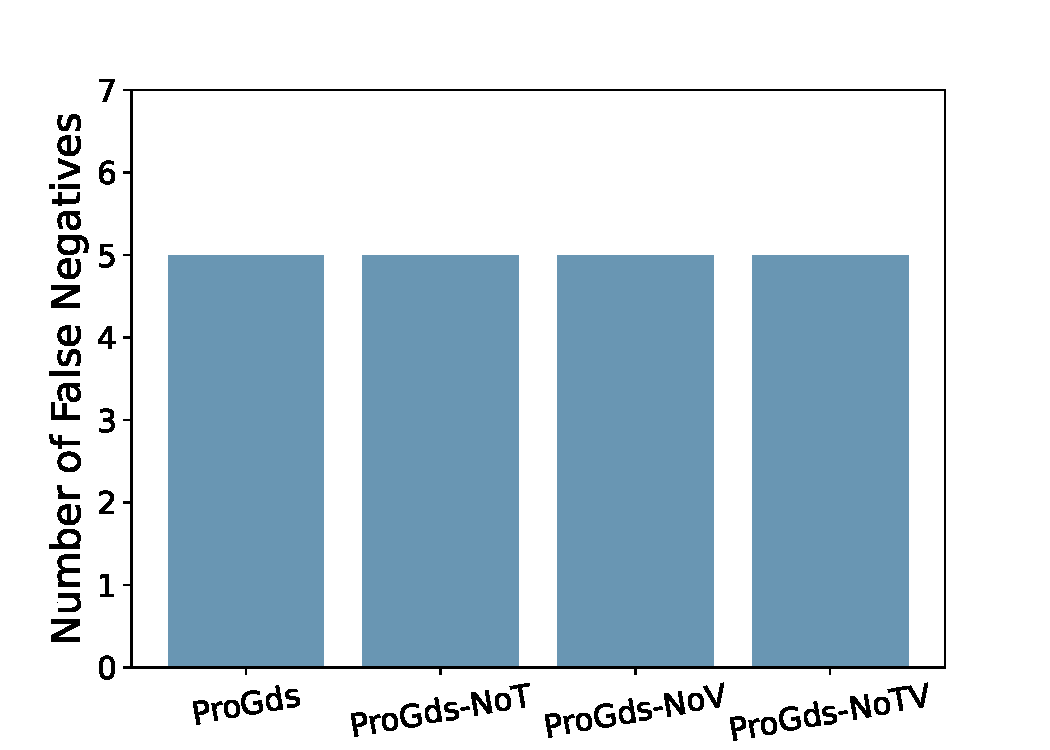
\includegraphics[width=\textwidth]{figs/FN.pdf}
        \caption{False Negative for In Attack Scenario}
        \label{fig:missed_attacks}
    \end{subfigure}
    \hfill
    \begin{subfigure}[b]{0.23\textwidth}
        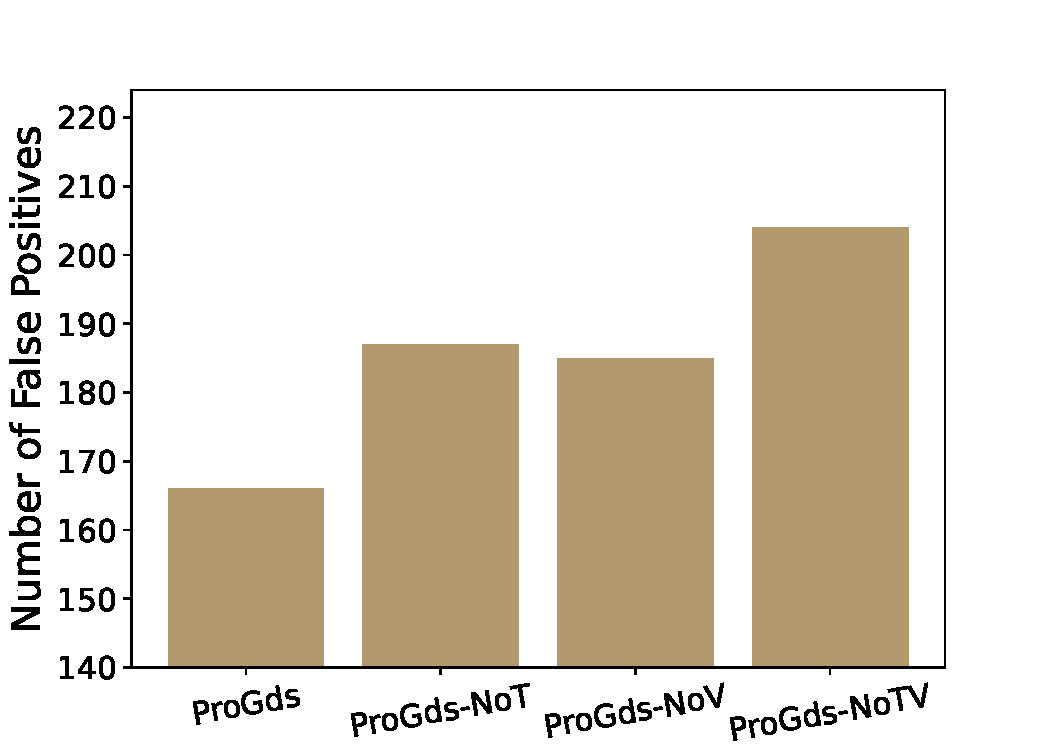
\includegraphics[width=\textwidth]{figs/FP.pdf}
        \caption{False Positives for Normal Scenario}
        \label{fig:false_positives}
    \end{subfigure}
    \caption{Comparison of different methods in terms of False Negative and false positives}
    \label{fig:comparison}
\end{figure}
We found no significant difference in attack scenarios between our method and the control method. Our approach, however, achieved the lowest false positive rate for normal scenarios.

In the following, examples are used to illustrate the role of adding behavior trees and validation links in reducing false positives.
Without the construction of the behavior tree, we obtain many constraints that are too broad.
For example, the behaviors that we mind and that \textit{svchost.exe} must obey when hosting certain services, like \textit{PhoneSvc} and \textit{NgcSvc}, must have behavior \textit{svchost.exe,CreateFile,*/localservice/appdata*}. However, for other services like the \textit{DHCP service}, this behavior isn't necessarily required.
These are not behaviors that all processes must adhere to, resulting in a high false positive rate when tested normally. 

We aim to demonstrate the effectiveness of our cross-session validation approach. To this end, we've introduced a novel validation method: employing three agents to engage in a debate to validate behaviors. From our experiments, it's evident that for actions that are undeniably factual, the three agents can reach a consensus after multiple rounds of debate. For instance, \textit{lsass.exe} will unquestionably load \textit{c:/windows/system32/lsasrv.dll}. On the other hand, for behaviors that aren't necessarily factual, the agents diverge in their opinions after several debate rounds and pinpoint the underlying reasons. For example, the behavior of \textit{sass.exe} with \textit{RegSetValue, hklm/system/currentcontrolset/control/lsa/} is not mandatory.



\subsection{Explanation Validation}
\label{sec-explanation-val}

Detection and interpretation are seamlessly integrated into our approach. The following sections explain how our method exposes attack behaviors and facilitates rapid verification and response to threats by security analysts.
To confirm the accuracy of the constraints we extracted, we searched Google, blogs, books, etc. In some public reports, we found consistency between their findings and our constraints.

There is some crucial document online\cite{nasbench}, including a technical document that outlines the execution paths and parent-child processes of 15 essential system processes. For instance, in the case of lsass.exe, the document indicates that its parent process is wininit.exe, it does not have a fixed child process, and its execution path is \textit{\%Systemroot\%/system32/lsass.exe}. It aligns with the knowledge we have gained through LLMs.
There is also document\cite{windows10dll} about static call relationship between Windows DLLs. \textit{Lsass.exe} will undoubtedly load \textit{lsasrv.dll}, and \textit{lsasrv.dll} and \textit{samsrv.dll} have a static link relationship. This knowledge also remains consistent with what we have learned through LLMs.
Through our analysis, it seems possible that the LLM might have learned from these documents. We have not found any specific references to support some illusions generated by LLMs.

% https://nasbench.medium.com/windows-system-processes-an-overview-for-blue-teams-42fa7a617920

% https://windows10dll.nirsoft.net/lsasrv_dll.html

\subsection{Real-world Validation}
\label{sec-real-world}

We collected some publicly available malicious software related to APTs, as shown in the Figure~\ref{tab:real_world}.
In some cases, such as for APT29, we were able to retrieve the original collected data directly, while in others we could only retrieve the dynamic execution logs from the VirusTotal sandbox. Using this real-world data, we wanted to verify the effectiveness of our method. As a result of the results, we can detect most types of stealth attacks using our method, including these four types of stealth attacks.

\begin{itemize}
    \item APT29 \cite{mitre_g0016}: We have analyzed malicious payloads associated with APT29, specifically focusing on \textit{python.exe}. According to the profile we constructed for a typical Python application, \textit{python.exe} would certainly load \textit{pythonxx.dll} and \textit{vcruntime140.dll}. However, in the dataset related to the malicious \textit{python.exe} used by APT29, we didn't find evidence of these two DLLs being loaded. This suggests that the \textit{python.exe} under scrutiny is likely not a standard or legitimate version.

    \item DCSrv\cite{checkpoint2021}: Moving on to the malware named DCSrv, we located this malicious software in the VirusTotal sandbox. We observed that it masquerades as \textit{svvhost.exe} with an execution path of \textit{C:/Users/user/Desktop/svvhost.exe}. \textit{Svchost.exe} has been obfuscated through string obfuscation, and its execution path is different from the typical \textit{svchost.exe} path.

    \item Sykipot\cite{att2023}: It appears that the malicious program Sykipot launches process injection attacks against \textit{firefox.exe}. The injected malicious dll is named \textit{wship4.dll}. There is no legitimate DLL by this name, but we did find \textit{wship6.dll}, which is related to IPv6 network operations. In order for \textit{wship6.dll} to interact correctly, \textit{WS2\_32.dll} must also be loaded. Furthermore, there was no indication that \textit{WS2\_32.dll} was loaded, indicating malicious activity.
\end{itemize}








